\documentclass[12pt]{article}

% This first part of the file is called the PREAMBLE. It includes
% customizations and command definitions. The preamble is everything
% between \documentclass and \begin{document}.

\usepackage[margin=0.75in]{geometry}  % set the margins to 1in on all sides
\usepackage{graphicx}              % to include figures
\usepackage{amsmath}               % great math stuff
\usepackage{amsfonts}              % for blackboard bold, etc
\usepackage{amsthm}                % better theorem environments


% various theorems, numbered by section

\newtheorem{thm}{Theorem}[section]
\newtheorem{lem}[thm]{Lemma}
\newtheorem{prop}[thm]{Proposition}
\newtheorem{cor}[thm]{Corollary}
\newtheorem{conj}[thm]{Conjecture}

\DeclareMathOperator{\id}{id}

\newcommand{\bd}[1]{\mathbf{#1}}  % for bolding symbols
\newcommand{\RR}{\mathbb{R}}      % for Real numbers
\newcommand{\ZZ}{\mathbb{Z}}      % for Integers
\newcommand{\col}[1]{\left[\begin{matrix} #1 \end{matrix} \right]}
\newcommand{\comb}[2]{\binom{#1^2 + #2^2}{#1+#2}}


\begin{document}


\title{REU Week 1 Writeup}

\author{Sayem Hoque\\
 \\ }

\maketitle
\date{}

\section{Different jitters}
Displacement of random horizontal lines in a video can cause the image stills to look jittered. This can be due to environmental or electromagnetic interference. The goal is to try to remove jitters from an image to find a better representation of what was actually occurring in the scene that is distorted. Jitters in an image can occur in any random fashion and different amounts of jittering could be occurring in different parts of the image. Because of this, we want our dejittering method to be general enough to work for any type of distortion. A normally distributed horizontal jitter was chosen to add to input images.
\begin{verbatim}
  % jitter.m

  displacement = round((2*lambda) * rand(1) - lambda)
  I(row, :) = [zeros(1, displacement), I(row, 1:c-displacement)];
\end{verbatim}
For every row, a normally distributed random number between - lambda and + lambda is generated as the displacement for that row. The image is shifted and padded with zeros on the left or right side (depending on which way the row is shifted).

\section{Heat equation, TVR, edge plots}

After each image is given a random jitter, Heat Equation, TVR, and resulting edge plots after each are done. In the results, these are described and some parameters were tweaked to try to replicate the results in the Bake and Shake paper. In the results, I was trying to show the advantages of using anisotropic diffusion (TVR) over isotropic diffusion (Heat Equation). In anisotropic diffusion, the major features such as edges and major lines in an image are left unmodified or less modified when allowing the image do diffuse out. In isotropic diffusion, the entire image is treated as the same during the diffusion process, regardless if there's an edge. \\

The hope is that even with the jittering of the image, the major features in the image will allow the anisotropic diffusion to let those features become more apparent again.

\section{Tests}

\subsection{Image 1}

\begin{figure}[ht!]
\centering
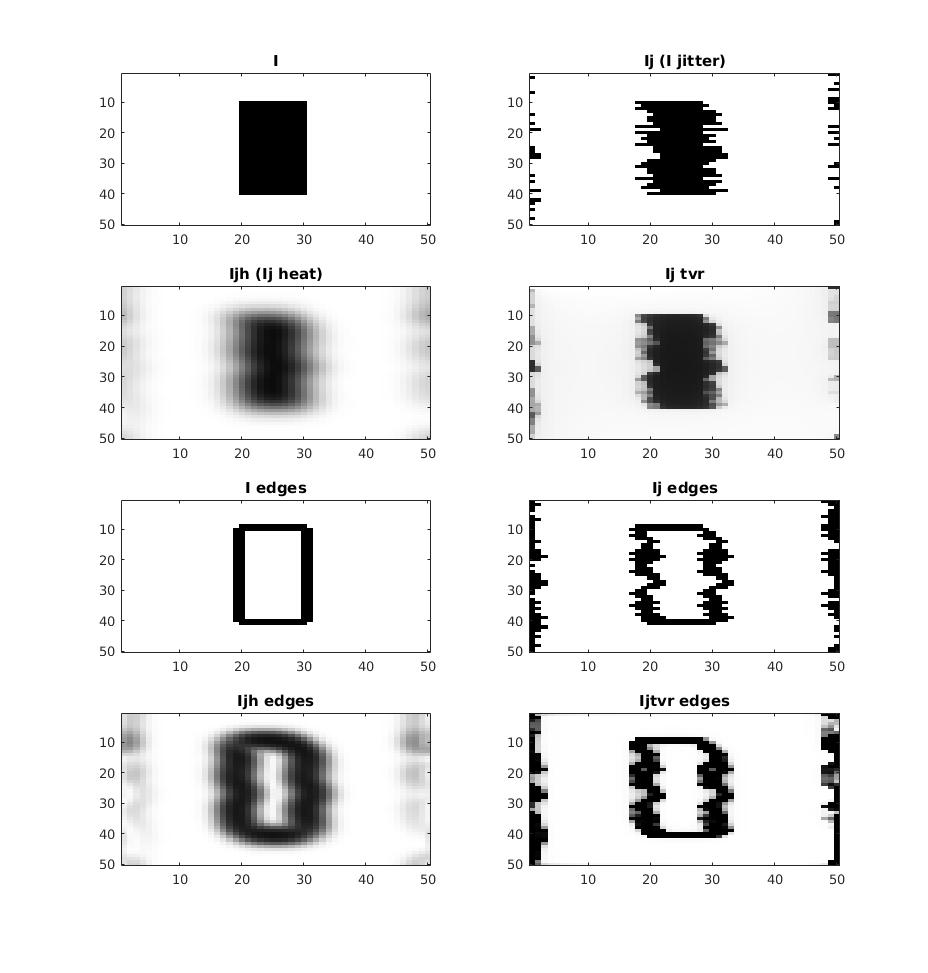
\includegraphics[scale=0.5]{one}
\end{figure}

\begin{figure}[ht!]
\centering
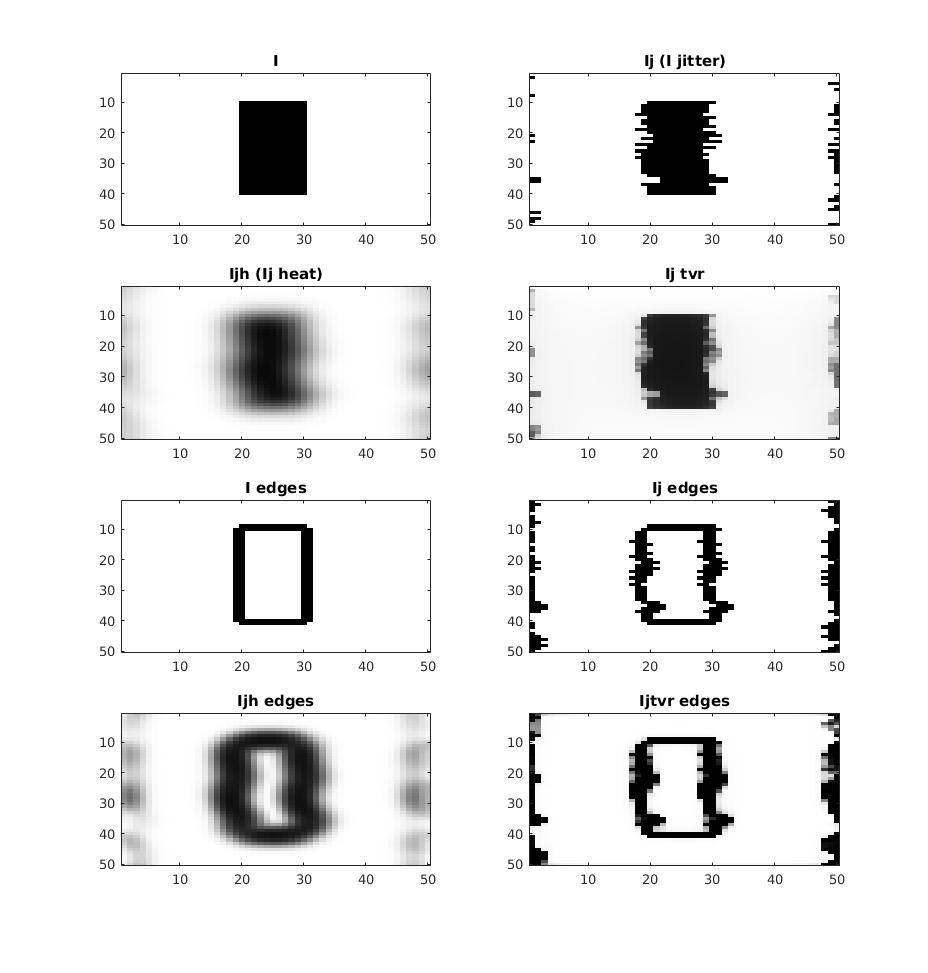
\includegraphics[scale=0.5]{two}
\end{figure}

In the two images, it can be seen how the isotropic diffusion rids the image more quickly of the edge data. Because of this, you can see when the findEdges function is run on the resulting image after heat, the edges are very fat. This is because edges are found where there are large differences in intensity. Because heatequation spreads out the edges so far, the area where there are large differences in intensity are spread out fat. In contrast, the tvr'ed image keeps the edges in tact better. The resulting edge plot is closer to the edge plot of the original image.

\begin{figure}[ht!]
\centering
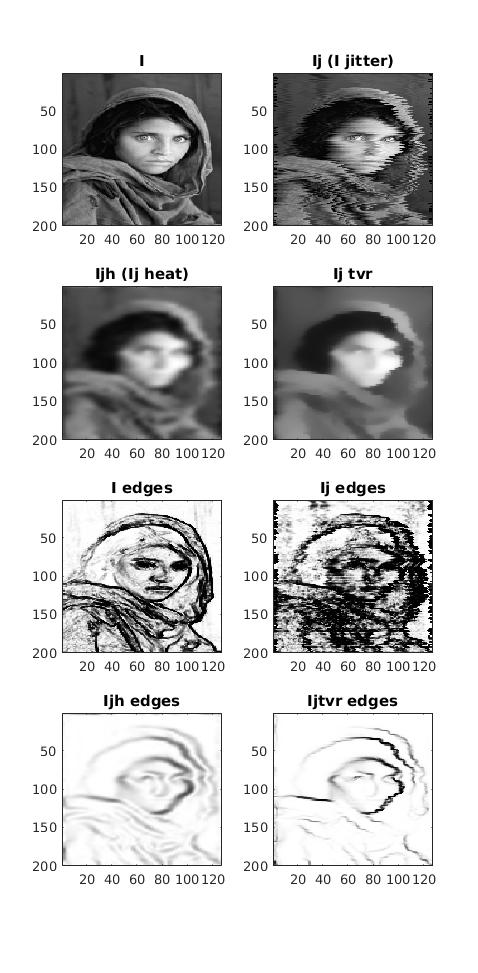
\includegraphics[scale=0.7]{three}
\end{figure}

\bibliography{writeup}
\bibliographystyle{plain}

\end{document}
